\documentclass{beamer}
\usepackage[utf8]{inputenc}

\usetheme{Copenhagen}


\usepackage{hyperref}      
\hypersetup{
	colorlinks=true,
	linkcolor=blue,
	filecolor=magenta,      
	urlcolor=blue,
	pdftitle={Overleaf Example},
	pdfpagemode=FullScreen
}  

\usepackage{amsmath}
\usepackage{amssymb} 
\usepackage{amsthm}  

\usepackage{float}
\usepackage{wrapfig}

\usepackage{geometry}
\usepackage{enumitem}

\begin{document}


\author{Thomas Arrous\and Gabin Dudillieu\and Yago Iglesias}
\title{How to learn without a brain}
\institute{Université Paris Cité}
\date{\today}


\begin{frame}[plain]
    \maketitle
\end{frame}

\begin{frame}{Introduction}{Fabrication d'un robot qui marche}
	\begin{center}
		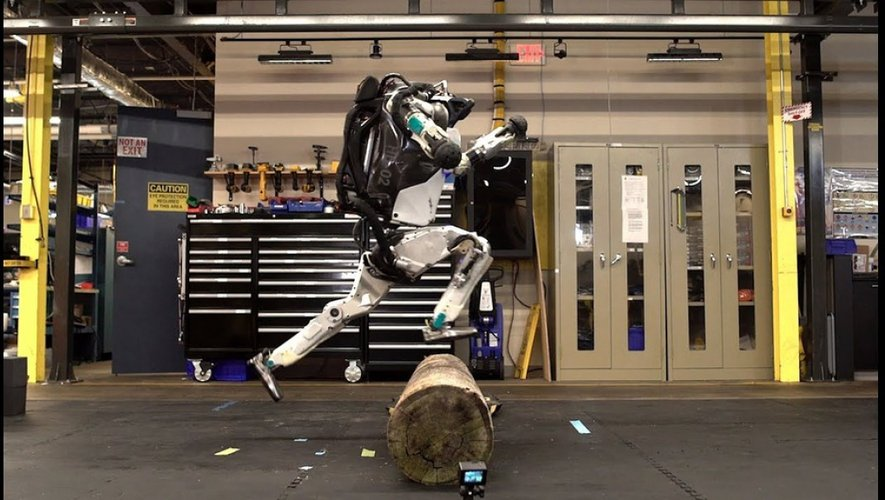
\includegraphics[width=10cm]{ressources/Intro/Robot saut.jpg}
	\end{center}
\end{frame}
\begin{frame}{Introduction}{Industrie pharmaceutique}
	\begin{center}
		\includegraphics[width=5cm]{ressources/Intro/médicaments.jpg}
		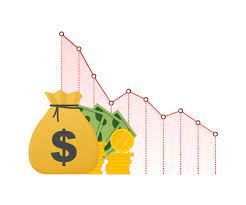
\includegraphics[width=5cm]{ressources/Intro/prix.jpg}
	\end{center}
\end{frame}
\begin{frame}{Introduction}{Des applications aux jeux}
	\begin{center}
		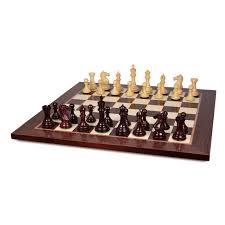
\includegraphics[width=5cm]{ressources/Intro/Echecs.jpg}
		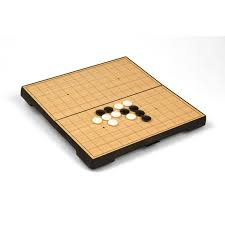
\includegraphics[width=5cm]{ressources/Intro/GO.jpg}
	\end{center}
\end{frame}
\begin{frame}{Introduction}{Sommaire}
	\begin{center}
		\begin{block}{Sommaire}
			\begin{itemize}[label=\textbullet, font=\LARGE \color{black}]
				\item Markov Decision Process(MDP)
				\item Monte Carlo Tree Search (MCTS)
				\item AlphaGo
			\end{itemize}
		\end{block}
	\end{center}
\end{frame}

\begin{frame}{Markov Decision Process(MDP)}{Qu'est ce que la décision de Markov}
	\begin{center}
		\begin{block}{Objectif}
			Lorsque le modèle rencontre un problème, il existe plusieurs manières de le résoudre. On cherche la meilleure solution. Lorsque l'on répète cette action, on appelle cela un processus de décision de Markov. 
		\end{block}
		\begin{block}{Principe}
			Un agent est capable de comprendre l’état dans lequel se trouve son environnement, et doit être en mesure de trouver une réponse afin de le modifier si besoin.
		\end{block}
	\end{center}
\end{frame}
\begin{frame}{Markov Decision Process(MDP)}{Fonctionnement de l'apprentissage par renforcement}
	\begin{center}
		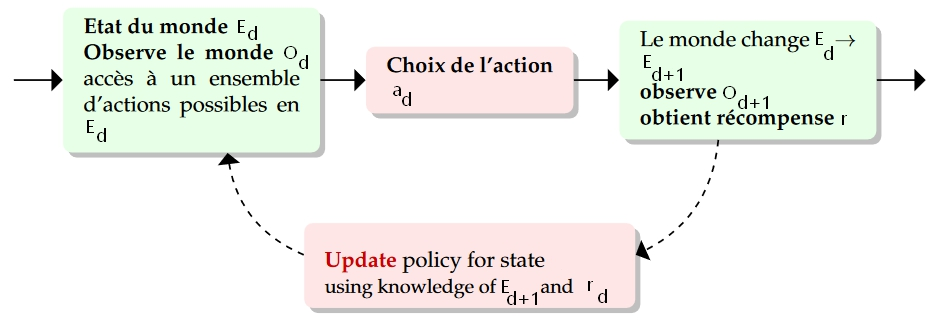
\includegraphics[width=10cm]{ressources/MDP/Fonctionnement.jpg}
	\end{center}
	\begin{block}{Objectif}
		Maximiser les récompenses.
	\end{block}
\end{frame}
\begin{frame}{Markov Decision Process(MDP)}{Qu'est ce qu'un état de Markov ?}
	\begin{center}
		
		\begin{block}{Visualisation}
			L'environnement est visualisable comme un automate probabilisé.
		\end{block}
		\begin{block}{Etat}
			On peut noter la probabilité d'arriver dans un état comme cela:\\
			Notons $E_{i}$ tous les états. Pour $i \in [1,d]$ avec $d$ l'indice du dernier état connu.\\
			Alors un état $E_{d+1}$ est dit de Markov si et seulement si :\\ 
			$$\mathbb{P}(E_{d+1} | E_{d}) = \mathbb{P}(E_{d+1} | E_{1}, ..., E_{d})$$\\
		\end{block}
		\begin{block}{Avantage}
			Ainsi l'état suivant ne dépend pas de tous les évènements qui ont précédé, mais juste de l'état précédent, comme aux échecs.
		\end{block}
	\end{center}
\end{frame}
\begin{frame}{Markov Decision Process(MDP)}{Maximiser les récompenses}
	\begin{center}
		
		\begin{block}{Fonction de récompense}
            \centering
			$R_t = \sum^{\infty}_{k=0}\gamma^{k}r_{t+k+1}$
		\end{block}
		\begin{block}{Explications}
			$r_{i}$ est la récompense obtenue au $i$-ième état.
			$\gamma$ est appelé facteur de dévaluation.\\
			$\gamma$ = 0 : l'agent ne voit rien, il ne veut que des récompenses immédiates.
			$0< \gamma <1$ cherche un équilibre entre la récompense immédiate et celles futures.
		\end{block}
		\begin{block}{Comment choisir le prochain état ?}
			La fonction valeur évalue la qualité d’un état, et ou d’une action. En se basant sur l’espérance du gain possible atteignable directement, et des gains qui pourront en découler. Ainsi elle permet de choisir l’action la plus favorable.
		\end{block}
	\end{center}
\end{frame}
\begin{frame}{Markov Decision Process(MDP)}{Chaines de Markov}
	\begin{center}
		
		\begin{center}{Un exemple d'automate}
			\includegraphics[width=9.8cm]{ressources/MDP/automate probabilisé.png}
		\end{center}
	\end{center}
\end{frame}
\begin{frame}{Markov Decision Process(MDP)}{Sous forme de matrice}
	\begin{center}
		\begin{center}{Matrice de transition}
			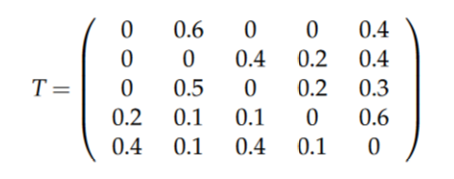
\includegraphics[width=10cm]{ressources/MDP/Matrice de transitions.png}
		\end{center}
	\end{center}
\end{frame}
\begin{frame}{Markov Decision Process(MDP)}{}
	\begin{center}
		\begin{block}{Markov Decision Process}
			Un Markov Decision Process est un tuple $<E,A,T,R,\gamma>$ où :\\
			$E$ est un ensemble fini d'états.\\
			$A$ est un ensemble fini d'actions.\\
			$T$ est une matrice de transition.\\
			$R$ sont les récompenses.\\
			$\gamma$ est le facteur de dévaluation.
		\end{block}
	\end{center}
\end{frame}

\begin{frame}{Monte Carlo Tree Search(MCTS)}{Qu'est-ce que le MCTS}
	\begin{block}{Définition MCTS}
		Le \textbf{MCTS} :
		\begin{itemize}
			\item - Est un algorithme de \textbf{recherche arborescente}.
			\item - Utilisé pour résoudre des problèmes afin de prendre une décision.
			\item - N'utilise pas de fonction d'évaluation heuristique.
			\item - \textbf{Parcours} les possibilités \textbf{aléatoirement} avec les données précédentes.
			\item - Utilise les méthodes de \textbf{Monte Carlo} pour améliorer son efficacité.
			\item - Possède des variantes (\textbf{Coulom}, \textbf{Kocsis}, \textbf{Szepesvari}, ...).
		\end{itemize}
	\end{block}
\end{frame}

\begin{frame}{Monte Carlo Tree Search(MCTS)}{Structure}
	\begin{block}{Arbre de recherche}
		\begin{itemize}
			\item Un \textbf{arbre de recherche} est une \textbf{modélisation} des possibilités de jeu pour la simulation.
			\item Un \textbf{noeud} représente un \textbf{état} du jeu.
			\item Chaque noeud possède deux informations :
			\item\begin{itemize}
				      \item - La \textbf{valeur} de sa position.
				      \item - Le \textbf{nombre de visites} de ce noeud dans la simulation.
			      \end{itemize}
			\item Chaque feuille de cet arbre représente soit un \textbf{noeud} dont les enfants n'ont pas encore été explorés, soit un \textbf{état final} de celui-ci.
		\end{itemize}
	\end{block}
\end{frame}

\begin{frame}{Monte Carlo Tree Search(MCTS)}{Structure}
	\begin{block}{Exemple d'arbre MCTS}
		\begin{center}
			\includegraphics[width=6cm]{ressources/MCTS/tree.png}
		\end{center}
	\end{block}
\end{frame}


\begin{frame}{Monte Carlo Tree Search(MCTS)}{Structure}
	\begin{block}{Plusieurs étapes}
		\begin{itemize}
			\item 1. \textbf{Sélection}
			\item 2. \textbf{Expansion}
			\item 3. \textbf{Simulation}
			\item 4. \textbf{Rétropropagation}
			\item Répété jusqu'à la prise de décision.
		\end{itemize}
		\begin{center}
			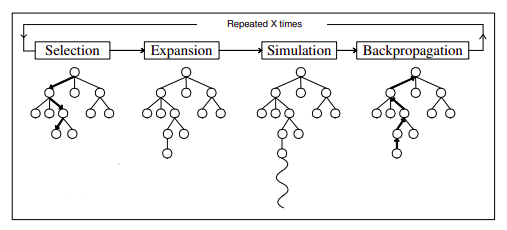
\includegraphics[width=8cm]{ressources/MCTS/MCTSEtapes}
		\end{center}
	\end{block}
\end{frame}

\begin{frame}{Monte Carlo Tree Search(MCTS)}{Sélection}
	\begin{block}{Fonctionnement de la sélection}
		\begin{columns}
			\begin{column}{7cm}
				\begin{itemize}
					\item - \textbf{Débute} à partir de la racine.
					\item \
					\item - Application \textbf{récursive} d'une \textbf{stratégie} de sélection pour \textbf{trouver} une feuille de l'arbre à étendre.
				\end{itemize}
			\end{column}
			\begin{column}{4cm}
				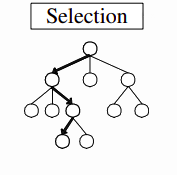
\includegraphics[width=3cm]{ressources/MCTS/Selection.png}
			\end{column}
		\end{columns}
	\end{block}
	\begin{block}{Stratégies de la sélection}
		\begin{itemize}
			\item Il existe plusieurs stratégies de sélection (\textbf{OMC}, \textbf{UCT}, \textbf{PBBM}, ...).

			\item Les \textbf{stratégies} les plus optimales font un consensus entre \textbf{exploitation} et \textbf{exploration}.
		\end{itemize}
	\end{block}
\end{frame}

\begin{frame}{Monte Carlo Tree Search(MCTS)}{Sélection}
	\begin{block}{Stratégie OMC (Objective Monte-Carlo)}
		\begin{itemize}
			\item ${U_{i}}$ une fonction d'urgence d'un mouvement avec :
			\item $U_{i} = erfc \left(\frac{v_{0} - v_{i}}{\sqrt{2}\sigma_{i}}\right)$
			\item $v_{0}$ la valeur du meilleur mouvement et $v_{j}$ la valeur du mouvement courant.
			\item $\sigma_{j}$ la déviation de $v_{j}$
			\item $erfc$ la fonction complémentaire d'erreur avec :
			\item $erfc(x) = 1 - \frac{2}{\sqrt{\pi}}\int_{x}^{\infty}e^{-u^{2}}$
			\item La probabilité $P_{m}$ pour chaque $m \in M$ avec :
			\item $P_{m} = \frac{U(m)}{\sum_{j \in S_{i}}^{}U(j)}$
			\item On choisit le prochain mouvement à simuler aléatoirement selon la probabilité $P_{m}$.
		\end{itemize}
	\end{block}
\end{frame}

\begin{frame}{Monte Carlo Tree Search(MCTS)}{Sélection}
	\begin{block}{Stratégie PBBM (Probability to be Better than Best Move)}
		\begin{itemize}
			\item Similitude avec la stratégie \textbf{OMC}.
			\item $U_{i}$ aussi une fonction d'urgence d'un mouvement avec :
			\item $U_{i} = \exp\left(-2.4\frac{v_{0} - v_{i}}{\sqrt{2(\sigma_{0}^2 + \sigma_{i}^2)}}\right) + \epsilon_{i}$
			\item $v_{0}$ la valeur du meilleur mouvement et $v_{i}$ la valeur du mouvement courant.
			\item $\sigma_{0}$ et $\sigma_{i}$ leur déviations.
			\item $\epsilon_ {i}$ une constante assurant que la fonction d'urgence ne soit pas égale à 0 avec :
			\item $\epsilon_ {i} = \frac{0.1 + 2^{-i} + a_{i}}{N}$
			\item $a_{i} = 1$ ou $0$ selon la situation.
		\end{itemize}
	\end{block}
\end{frame}

\begin{frame}{Monte Carlo Tree Search(MCTS)}{Sélection}
	\begin{block}{Stratégie UCT (Upper Confidence bounds applied to Trees)}
		\begin{itemize}
			\item La stratégie \textbf{UCT} sélectionne un noeud $k$ fils du noeud $p$ qui satisfait la formule suivante :
			      $$k \in argmax_{i\in I}\left(v_{i} + C \times \sqrt{\frac{\ln n_{p}}{n_{i}}}\right)$$
			\item $I$ un set de noeuds atteignable par le noeud $p$.
			\item $v_{i}$ la valeur du noeud $i$
			\item $n_{p}$ et $n_{p}$ le nombre de fois que les noeuds $p$ et $i$ on été visités.
			\item $C$ une constante.
		\end{itemize}
	\end{block}
\end{frame}

\begin{frame}{Monte Carlo Tree Search(MCTS)}{Sélection}
	\begin{block}{Stratégie UCB1-TUNED}
		\begin{itemize}
			\item Variante de la stratégie \textbf{UCT} qui sélectionne un noeud $k$ fils du noeud $p$ qui satisfait la formule suivante :
			      $$k \in argmax_{i\in I}\left(v_{i} + C \times \sqrt{\frac{\ln n_{p}}{n_{i}}\times \min(\frac{1}{4}, V_{i}(n_{i}))}\right)$$
			\item avec $V_{i}$ une estimation de la borne supérieur de la variance de $v_{i}$ avec comme formule :
			      $$V_{i}(n_{i}) = \frac{1}{n_{i}}\sum_{t=1}^{n_{i}}R_{i,t,j}^2 - v_{i}^2 + \sqrt{\frac{2\ln n_{p}}{n_{i}}}$$
			\item $R_{i,t,k}$ la $t$-ième récompense obtenu au noeud $i$ pour le joueur $j$
		\end{itemize}
	\end{block}
\end{frame}

\begin{frame}{Monte Carlo Tree Search(MCTS)}{Expansion}
	\begin{block}{Fonctionnement Expansion}
		\begin{columns}
			\begin{column}{8cm}
				\begin{itemize}
					\item - \textbf{Dépend} des règles du jeu.
					\item - \textbf{Crée} un noeud à partir du noeud sélectionné si celui-ci n'est pas final.
					\item \
					\item Tout les résultats ne sont pas gardés en mémoire.
				\end{itemize}
			\end{column}
			\begin{column}{4cm}
				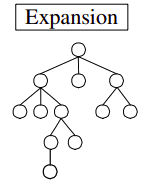
\includegraphics[width=2.5cm]{ressources/MCTS/Expansion.png}
			\end{column}
		\end{columns}
	\end{block}
	\begin{block}{Stratégies de l'expansion}
		\begin{itemize}
			\item Il existe \textbf{plusieurs stratégies} pour choisir les noeuds à garder :
			\item - \textbf{Garder seulement} un noeud par jeu simulé.
			\item - \textbf{Continuer} à \textbf{stocker} les enfants d'un noeud jusqu'à un nombre \textbf{limité} de simulations.
		\end{itemize}
	\end{block}
\end{frame}

\begin{frame}{Monte Carlo Tree Search(MCTS)}{Simulation}
	\begin{block}{Fonctionnement de la simulation}
		\begin{columns}
			\begin{column}{7cm}
				\begin{itemize}
					\item - \textbf{Réalise} une \textbf{simulation} d'une partie aléatoirement à partir du noeud étendu.
					\item \
					\item - \textbf{Continue} de \textbf{parcourir} des états de jeu jusqu'à obtenir un résultat.

				\end{itemize}
			\end{column}
			\begin{column}{3cm}
				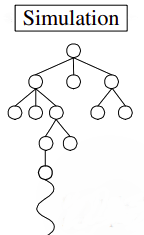
\includegraphics[width=2.2cm]{ressources/MCTS/Simulation.png}
			\end{column}
		\end{columns}
	\end{block}
	\begin{block}{Stratégies de la simulation}
		Il existe des \textbf{stratégies} de simulation qui sont difficile à définir.

		Ces \textbf{stratégies} peuvent utiliser des \textbf{connaissances acquises} du jeu (patterns, considérations, ...)
	\end{block}
\end{frame}

\begin{frame}{Monte Carlo Tree Search(MCTS)}{Simulation}
	\begin{block}{Statégie Sequence-like Simulation}
		\begin{columns}
			\begin{column}{8cm}
				\begin{itemize}
					\item Cette stratégie est adapté au jeu de GO, et consiste à :
					\item - \textbf{Sélectionner} chaque coup à proximité du dernier coup joué $c_{0}$ avec $E$ l'ensemble des coups adjacents.
					\item - \textbf{Choisir} un coup à jouer dans $E$, en cherchant des motifs de jeu de taille 3x3 à une distance 1 de Manhattan avec $c_{0}$.
					\item - Si plusieurs motifs correspondent :
					      \textbf{choix aléatoire parmi eux}.
					\item - Si aucun est reconnu :
					      \textbf{choix aléatoire parmi tous}.
				\end{itemize}
			\end{column}
			\begin{column}{3cm}
				\vspace{1cm}
				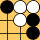
\includegraphics[width=2cm]{ressources/MCTS/3x3GridGo.png}
				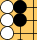
\includegraphics[width=2cm]{ressources/MCTS/3x3GridGo2.png}
			\end{column}
		\end{columns}
	\end{block}\end{frame}

\begin{frame}{Monte Carlo Tree Search(MCTS)}{Rétropropagation}
	\begin{block}{Fonctionnement de la rétropropagation}
		\begin{columns}
			\begin{column}{8cm}
				\begin{itemize}
					\item - \textbf{Propage} l'information aux \textbf{parents} du noeud récursivement avec le résultat de la simulation.
					\item - \textbf{Se propage} jusqu'au noeud le plus haut pour \textbf{diffuser} les nouvelles informations.
					\item - \textbf{Change} la valeur des noeuds visités.
					\item - \textbf{Garde} en mémoire le nombre de visites.
					\item  On pose $R_{i}$ le résultat d'une partie pour interpréter le résultat :

					      - $R_{i} = +1$ si l'IA gagne

					      - $R_{i} = -1$ si l'IA perd

					      - $R_{i} = 0$ si égalité.
				\end{itemize}
			\end{column}
			\begin{column}{4cm}
				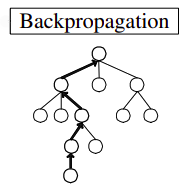
\includegraphics[width=3cm]{ressources/MCTS/Backpropagation.png}
			\end{column}
		\end{columns}
	\end{block}
\end{frame}

\begin{frame}{Monte Carlo Tree Search(MCTS)}{Stratégie Rétropropagation}
	\begin{block}{Stratégies de la rétropropagation}
		\begin{itemize}
			\item \textbf{Moyenne} : Prend la moyenne des résultats : $v_{i} = \frac{\sum_{i}^{}R_{i}}{n_{i}}$ avec $v_{i}$ la valeur du noeud et $n_i$ le nombre de fois qu'il a été visité.
			\item \textbf{Max} : Prend le max des résultats des enfants.
			\item \textbf{Moyenne informée} : Attribue de plus grandes valeurs aux meilleurs résultats.
			      On a : $v_{i} = \frac{\sum_{j}^{}(v_{j}\times n_{j}\times U_{j})}{\sum_{j}^{}(n_{j}\times U_{j})}$ avec $U_{j}$ la fonction d'urgence utilisée pour la stratégie de sélection OMC.
		\end{itemize}
	\end{block}
\end{frame}

\begin{frame}{Monte Carlo Tree Search(MCTS)}{Choix du mouvement final}
	\begin{block}{Statégies du choix du mouvement final}
		\begin{itemize}
			\item \textbf{Maximum des noeuds}: On prend le noeud qui a la plus grande valeur.
			\item \textbf{Noeud le plus robuste}: On prend le noeud qui a été visité le plus de fois.
			\item \textbf{Mix}: On prend le noeud qui est à la fois le maximum et à la fois le plus robuste.
			\item \textbf{Noeud le plus sécurisé}: On prend le noeud qui maximise une borne de confiance.
		\end{itemize}
	\end{block}
\end{frame}

\begin{frame}{Monte Carlo Tree Search(MCTS)}{Application}
	\begin{block}{Applications du MCTS}
		\begin{itemize}
			\item Le \textbf{MCTS} a été une \textbf{révolution} pour les jeux à deux joueurs.
			\item \textbf{Mogo Titan}, un programme \textbf{MCTS}, a été le premier à avoir battu un joueur professionnel de Go avec contrainte (7 pierres d'handicap).
			\item Il est utilisé par des programmes comme \textbf{MOGO}, \textbf{CRAZY STONE}, \textbf{FUEGO}, ...
			\item \textbf{AlphaGo} utilise aussi le MCTS pour sa recherche de coup.
		\end{itemize}
	\end{block}
\end{frame}


\begin{frame}{AlphaGo}
    \begin{center}

        
\includegraphics[width=5cm]{ressources/AlphaGo/AlphaGoLogo}
    \end{center}
    \begin{block}{}
        \begin{itemize}
            \item Développé par Google DeepMind
            \item En mars 2016 \textbf{AlphaGo} a battu Lee Sedol, l'un des meilleurs joueurs de Go
        \end{itemize}
    \end{block}
    \begin{exampleblock}{\textbf{Technologies utilisées:}}
        \begin{itemize}
            \item Apprentissage par renforcement
            \item Réseaux de neurones profonds
            \item Monte Carlo Tree Search
        \end{itemize}
    \end{exampleblock}
\end{frame}



\begin{frame}{AlphaGo}{Composants}
    \begin{center}
        \textbf{Composants}
    \end{center}
    \begin{columns}[t]
        \begin{column}{.3\textwidth}
            \begin{block}{Policy network}
                Réseau neuronal qui renvoie une \textbf{distribution de probabilité} sur le coups possibles.
            \end{block}
        \end{column}
        \begin{column}{.3\textwidth}
            \begin{block}{Value Network}
                Réseau neuronal chargé d'estimer la \textbf{valeur} d'une position.            \end{block}
        \end{column}
        \begin{column}{.3\textwidth}
            \begin{block}{Fast Rollout policy}
                Politique plus simple que les autres qui permet une \textbf{simulation rapide} du reste de la partie.
            \end{block}
        \end{column}
    \end{columns}
\end{frame}

\begin{frame}{AlphaGo}{Entraînement des réseaux neuronales}
    \begin{center}
        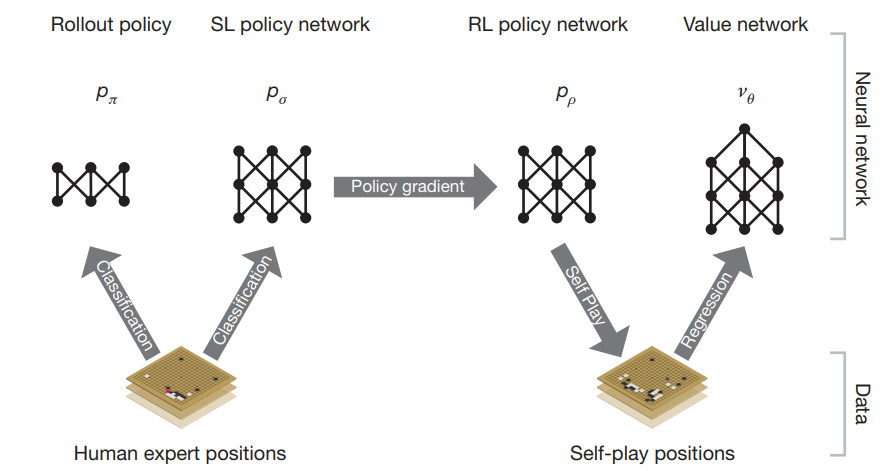
\includegraphics[width=7cm]{ressources/AlphaGo/Entrainement}
        \begin{columns}[t]
            \begin{column}{.4\textwidth}
                \begin{block}{Avec un modèle}
                    Entraînement d'un réseau \textbf{supervisé} (SL).
                \end{block}
            \end{column}
            \begin{column}{.4\textwidth}
                \begin{block}{Self-play}
                    Apprentissage par renforcement à partir du SL en jouant des parties \textbf{contre soi-même}.
                \end{block}
            \end{column}
        \end{columns}

    \end{center}
\end{frame}


\begin{frame}{AlphaGo}{Apprentissage avec un modèle (SL)}
    \begin{center}

        \begin{block}{Objectif}
            Modèle qui prédit, à partir d'un état $s$, l'action $a$ qu'un joueur professionnel aurait fait.
        \end{block}
        \vspace{1cm}
        \begin{block}{Solution}
            Réseau neuronal convolutif avec 13 couches.
            Entraînement initial \textbf{supervisé} à partir de parties jouées par des professionnels (30 million de positions différentes).
        \end{block}
    \end{center}
\end{frame}

\begin{frame}{AlphaGo}{Apprentissage avec un modèle (SL)}
    \begin{block}{Resultat}
        Politique $p_\sigma$, avec $\sigma$ les paramètres (les poids) du réseau.
        Temps d'évaluation de l'ordre de \textbf{3 ms} avec une précision de \textbf{57.0\%}.
    \end{block}
    \begin{center}
        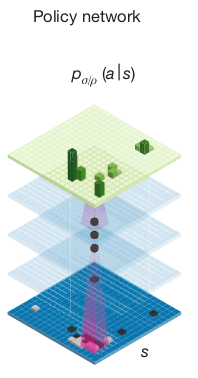
\includegraphics[scale=0.4]{ressources/AlphaGo/Policy_Network}
    \end{center}
\end{frame}

\begin{frame}{AlphaGo}{Self-play}
    \begin{block}{Objectif}
        \begin{center}
            Trouver une politique \textbf{meilleure} que $p_\sigma$.
        \end{center}
    \end{block}

    \begin{block}{Solution}
        \begin{itemize}
            \item Entraînement par renforcement en jouant des parties contre \textbf{soi-même}.
            \item Système de recompense simple : +1 si victoire et -1 si défaite.
            \item Structure \textbf{égale à celle du SL}, avec une politique $p_\rho$, avec des poids initiales égaux à $\sigma$.
            \item Parties entre la version actuelle de l'agent et une \textbf{version antérieure aléatoire}.
            \item Taux de réussite contre le SL : \textbf{80\%}.
        \end{itemize}
    \end{block}
\end{frame}


\begin{frame}{AlphaGo}{Value network}
    La \textbf{value network} nous permet d'estimer la \textbf{valeur} d'une position.
    \begin{block}{Modèle théorique}
        On définit $v^p$ comme la fonction qui prédit le résultat de la partie en partant de la position $s$ suivant la politique $p$.$$v^p(s) = \mathbb{E}[z_t|s_t=s, a_{t,\dots,T}\sim p]$$
        L'idéal est de trouver $v^*$, la fonction de valeur optimale, mais c'est impossible.
        On décide d'utiliser la meilleur politique qu'on connaît: $p_\rho$, ainsi on peut \textbf{approximer} la valeur de $v^*$. $$v_\theta(s) \approx v^{p_\rho}(s) \approx v^*(s)$$
    \end{block}
\end{frame}

\begin{frame}{AlphaGo}{Value network}
    \begin{block}{Solution}
        \begin{itemize}
            \item Utiliser un réseau de neurones profond.
            \item Sa structure est la même que celle du RL mais avec \textbf{une seule sortie} et il est entraîné sur la RL.
        \end{itemize}
    \end{block}
    \begin{center}
        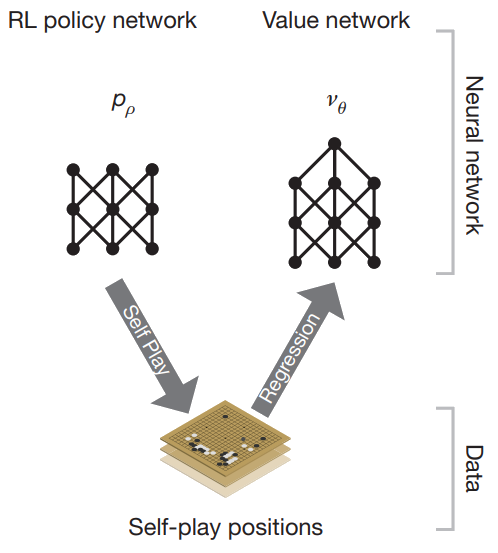
\includegraphics[width=5cm, height=5.2cm]{ressources/AlphaGo/RL_and_VN}
    \end{center}
\end{frame}

\begin{frame}{AlphaGo}{Fast rollout policy}
    \begin{block}{Objectif}
        \begin{center}
            Politique \textbf{rapide} qui permet de \textbf{simuler} le reste de la partie.
        \end{center}
    \end{block}
    \begin{block}{Solution}
        \begin{itemize}
            \item
            \item Entraîné avec le même modèle que le SL.
            \item Architecture beaucoup plus simple.
            \item Politique $p_\pi$.
            \item Précision de \textbf{24.2\%}.
            \item Temps d'évaluation de \textbf{2} $\boldsymbol{\mu s}$.
        \end{itemize}
    \end{block}
\end{frame}


\begin{frame}{AlphaGo}{MCTS}
    \begin{center}
        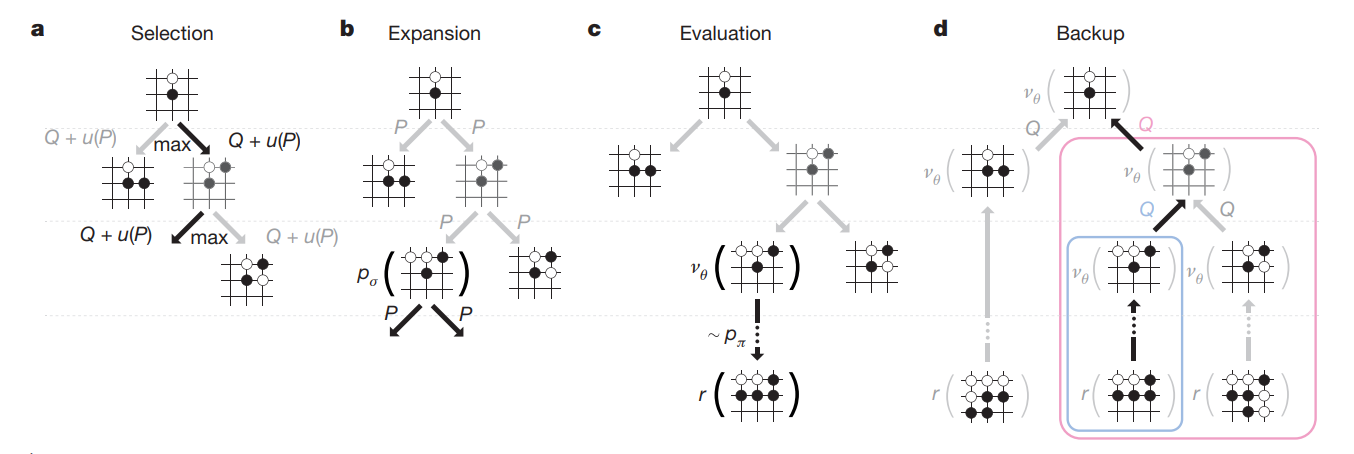
\includegraphics[width=10.5cm, height=3.8cm]{ressources/AlphaGo/MCTS_AlphaGo}
        \begin{block}{ Fonctions du MCTS }
            \begin{columns}[t]
                \begin{column}{0.45\textwidth}
                    Calcul de la valeur de l'action $a$ dans la position $s$.
                    $$Q(s,a) = \frac{1}{N(s,a)}\sum\limits_{i=1}^{n} 1_{s,a,i} V(s_L)$$

                \end{column}
                \begin{column}{0.45\textwidth}
                    Fonction bonus inversement proportionnelle aux visites du noeud.
                    $$u(s,a) \propto \frac{P(s,a)}{1+N(s,a)}$$
                \end{column}
            \end{columns}
        \end{block}
    \end{center}
\end{frame}

\begin{frame}{AlphaGo}{MCTS}
    \begin{center}
        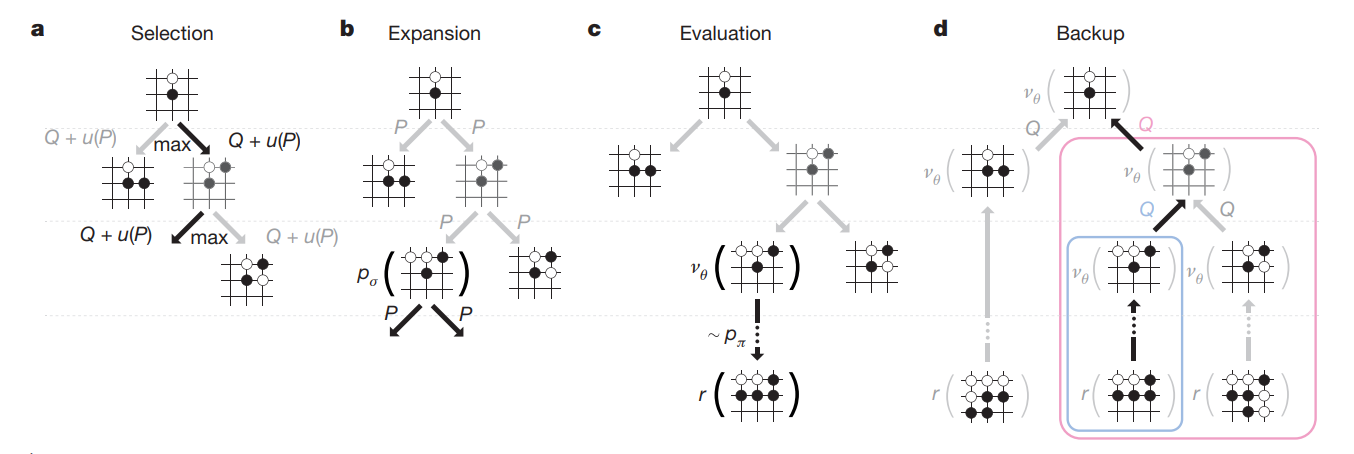
\includegraphics[width=10.5cm, height=3.8cm]{ressources/AlphaGo/MCTS_AlphaGo}
        \begin{block}{ Fonctions du MCTS }
            \begin{columns}[t]
                \begin{column}{0.45\textwidth}
                    Calcul de la valeur de l'action $a$ dans la position $s$, selon la politique $p_\sigma$:
                    $$P(s,a) = p_\sigma(a|s)$$

                \end{column}
                \begin{column}{0.45\textwidth}
                    Calcul du nombre de visites du noeud:
                    $$N (s,a) = \sum\limits_{i=1}^{n} 1_{s,a,i} $$
                \end{column}

            \end{columns}
        \end{block}

    \end{center}
\end{frame}

\begin{frame}{AlphaGo}{MCTS}
    \begin{center}
        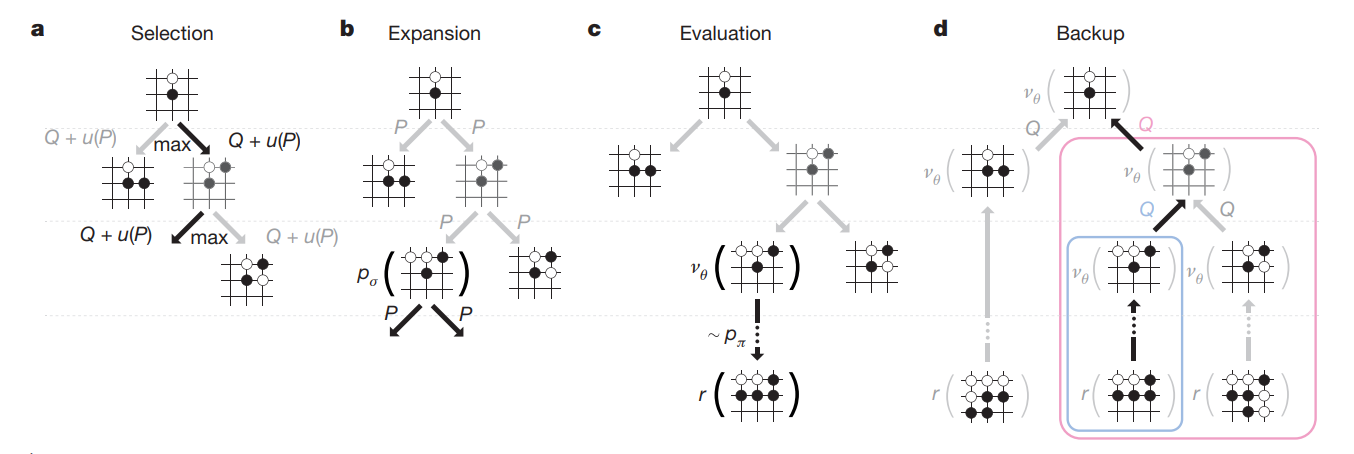
\includegraphics[width=10.5cm, height=3.8cm]{ressources/AlphaGo/MCTS_AlphaGo}
        \begin{block}{ Fonctions du MCTS }
            Valeur de la position $s_L$:
            $$V(s_L)=(1-\lambda)v_\theta(s_L) + \lambda z_L \mbox{, avec } \lambda \in [0,1]$$
        \end{block}
    \end{center}
\end{frame}

\begin{frame}{AlphaGo}{Résultats}
    \begin{columns}[t]
        \begin{column}{.4\textwidth}
            \vspace{-1.5cm}
            \begin{figure}
                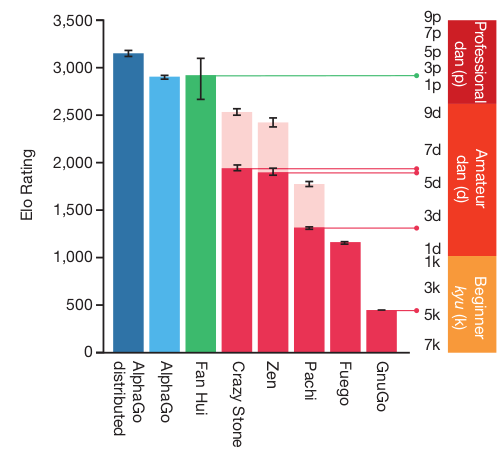
\includegraphics[scale=0.3]{ressources/AlphaGo/AlphaGovsShit.png}
                Elo de AlphaGo comparé à d'autres IA
            \end{figure}
        \end{column}
        \begin{column}{.4\textwidth}
            \begin{figure}
                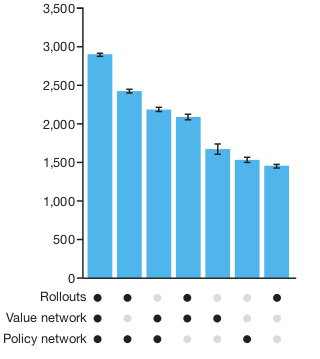
\includegraphics[scale=0.3]{ressources/AlphaGo/comparaison_different_models}
                \\
                Elo de AlphaGo selon les composants utilisés
            \end{figure}
        \end{column}
    \end{columns}
\end{frame}


\begin{frame}{Conclusion}{}
	\begin{center}
		
\includegraphics[width=10cm]{ressources/Conclusion/BrainStormRobot.jpg}
	\end{center}
\end{frame}

\begin{frame}{Conclusion}{}
	\begin{center}
		\begin{LARGE}
			Avez-vous des questions ?
		\end{LARGE}
	\end{center}
\end{frame}
\begin{frame}{Références}
    \begin{block}{Markov decision process}
        \href{https://members.loria.fr/ADutech/Papier/dutech_selectifPOMDP_RIA03.pdf}{Alain Dutech et Manuel Samuelides (2003)}
    \end{block}
    \begin{block}{Monte Carlo Tree Search}
        \href{https://project.dke.maastrichtuniversity.nl/games/files/phd/Chaslot_thesis.pdf}{Chaslot thesis}\\
        \href{https://helios2.mi.parisdescartes.fr/~bouzy/publications/Chaslot-MCStrategiesComputerGo-BNAIC06.pdf}{Chaslot strategies}\\
        \href{https://hal.inria.fr/inria-00116992/document}{INRIA paper}
    \end{block}
    \begin{block}{AlphaGo}
        \href{https://www.nature.com/articles/nature16961#citeas}{Nature AlphaGo paper}\\
        \href{https://arxiv.org/abs/1712.01815}{AlphaGo Zero paper}
    \end{block}
\end{frame}



\end{document}
